%% ---------------------------------------------------------------------
%% Copyright 2014, Thales, IGN, Rémi Cura
%% 
%% This file contains the introduction of article
%% ---------------------------------------------------------------------


\section{Introduction}

\begin{figure*}[t!]
	\begin{center}
		\fbox{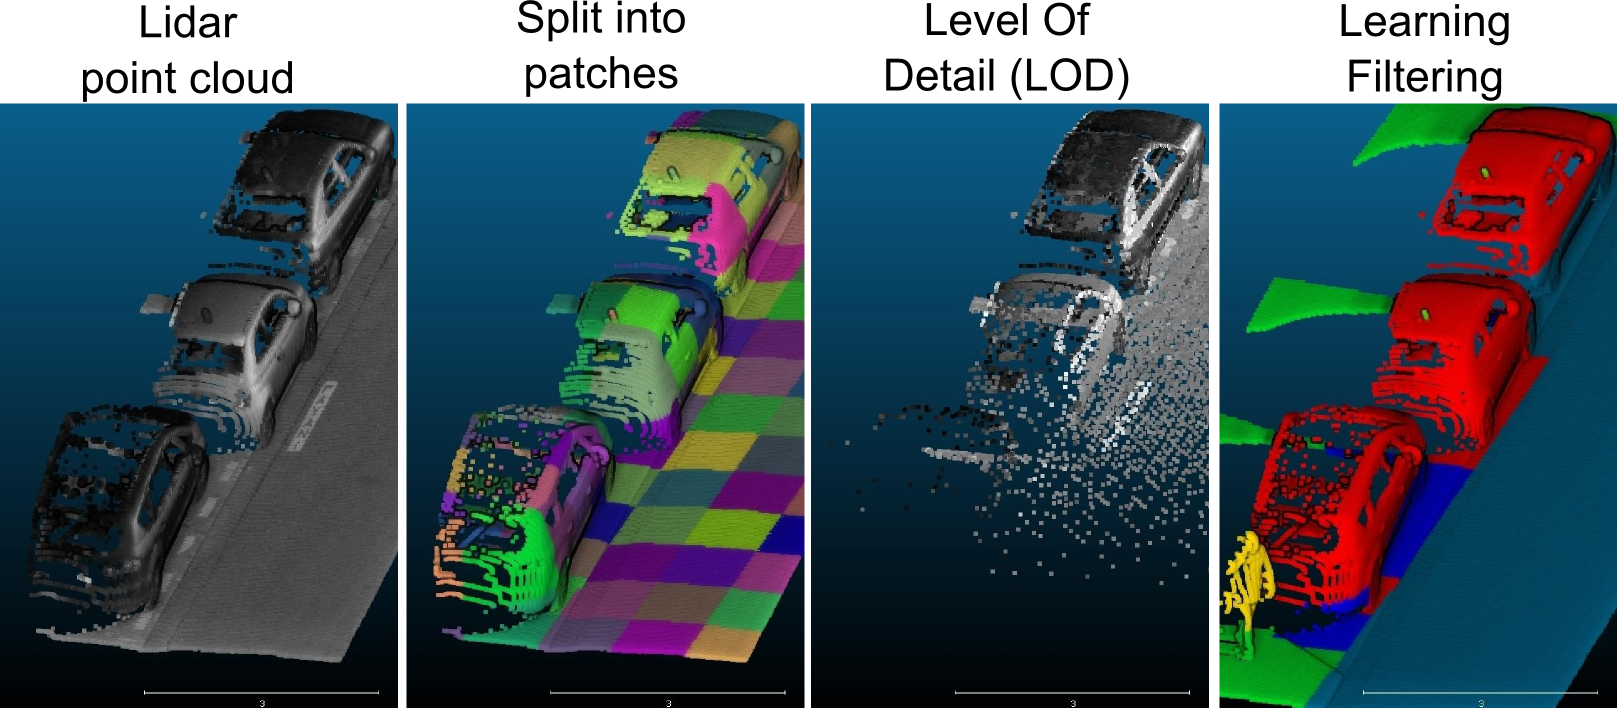
\includegraphics[width=\textwidth,keepaspectratio ]{./illustrations/banner_for_paper.png}}
		\caption{Data flow : a Lidar point cloud (1), is split it into patches (2) , patches are re-ordered to obtain free LOD (3 : a gradient of LOD here). Lastly the ordering is used as a feature for learning and efficient filtering (4) } 
		\label{fig:banner_image}
	\end{center}
\end{figure*} 

	\subsection{Problem}  
		Point cloud data is becoming more and more common. Following the same trend, the acquisition frequency and precision of the Lidar device are also increasing.
		Thus point cloud processing is entering in the Big Data realm.
		
		Yet the usage of point cloud data is also spreading and going out of their traditional user communities. 
		Lidar are now commonly used by non-specialized users. 
		
		
		For many usages, having the raw, complete point cloud is unnecessary, or even damageable. In these cases, only a well chosen sub-sample of the data, or a more abstract representation are needed.
		Thus we deal with a simpler version of a problem common for Geographical Information System (GIS): how to generalize information, that is reduce the details of the data while retaining its principal organization, with huge data sets?
		
		Such a problematic is very common, and we could consider it as a case of compression, clustering, dimensionality reduction, etc.
		
		In \cite{cura2015} we proposed to use the Point Cloud Server (PCS) to store groups of points and use generalisation for those groups tailored for special use case. For instance the groups of points may be generalised by planes, which would be well adapted for fast registration.
		
		Yet those generalisations introduce more abstract data than point cloud, and necessitate ad-hoc methods to be used.
		
		In simplest use case we may simply want to abstract the data by reducing the number of points.
		This particular problem applied to visualisation is commonly called Level Of Details (LOD, cf \href{banner_image}{figure ~\ref{fig:banner_image}}).
		
		The problem is then how to reduce the amount of points while preserving the geometric characteristics of the underlying sensed object, in an efficient manner, and while being robust to the way the sensing was done?
		Indeed LOD approaches sacrifices of a part of information in exchange of a massive reduction of data size which is necessary for efficient usage/visualisation. In this regard, a LOD method must by nature be efficient, or the information loss would be pointless.
		
		We can see point cloud as a sampling of a surface (or volume) of the sensed object. This sensing may be structured for the sensing device (for instance a Lidar may sense point using a constant angle), but not necessary for the sensed object (see figure \ref{fig:irregular_sampling})
		\myimage{"./illustrations/problem_in_sampling/regular_vs_irregular_sampling"}{Regular sensing does not imply regular sampling}{fig:irregular_sampling}.
		

	\subsection{State of the Art} 
		
		Maybe the most basic method to reduce the number of points is to perform a subsampling of the points. For instance, taking one point every ten would reduce the dataset by an order of magnitude.
		However this may introduce aliasing issue if the data is regularly sampled. We may solve this by randomly choosing the points to keep,
		yet those points may not be the best chosen to represent the sensed object, and such random sub sampling would be sensible to variation of points density (points in the denser part would be more chosen than points in less-dense part).
		
		
		One way to tackle data size is to use a Level Of Detail strategy. Octree methods have been common in computer graphics for several decades \cite{Meagher1982}. They are used in many methods to speed computing, or compress data, like in the work of \cite{Schnabel2006,Huang2006} (which have not been designed to scale).
		
		\cite{Elseberg2013} give a good overview of octree usage for point clouds. Their method proposes to directly store the points and octree in a file. They explore many applications that could benefit from our method (visual LOD, registration, processing). We share many objectives. It is an extremely effective approach that also enables visual LOD, but is very specialized on geometry. In particular, this method is not integrated with other GIS data (Geographical Information System), point cloud fast querying is not possible on attributes or metadata, and point cloud format is extremely specific.
		\\
		Another orthogonal way is to not use file, but store point cloud in DBMS.  \cite{vanOosterom2014} implements such system at very big scale and discuss how it can answer to various need. This approach has gained recent interest (\cite{pgPointCloud2014}) because it is generic, it scales naturally to very large data set and is easier to implement than starting from scratch. We also observe that most of Big Data system use methods from the DBMS world.
		\\ 
		\cite{Demantke2014} introduces a sophisticated per-point dimensionality descriptor, which is used to find optimal neighbourhood size. A main difference is that this feature is computed for each point (thus is extremely costly to compute), and that dimensionality is influenced by density variation.
		
		Random Forest method started with \cite{Amit97shapequantization} and theorized by \cite{Breiman2001} and has been very popular since then. They are for instance used by \cite{Golovinskiy2009} who perform object detection, segmentation and classification. They analyse separately each task on an urban data set, thus providing valuable comparison. Their method is uniquely dedicated to this task, like \cite{Serna2014} who provide another method and a state of the art of the segmentation/classification subject.
		Both of this methods are in fact 2D methods, working on an elevation image obtained by projecting the point cloud. However we observe that street point clouds are dominated by vertical surfaces, like building (about 70\% in Paris data set). Our method is fully 3D and can then easily be used to detect vertical object details, like windows or doors on buildings.
		 
	
	\subsection{Contribution}
		This paper re-uses and combines existing and well established methods with a focus on simplicity and efficiency. As such, all the methods are tested on billions scale point cloud, and are Open Source for sake of reproducibility test and improvements.
		We propose a simple method that enables portable, computation-free, geometrical Level Of Detail.
		Our first contribution is to propose to store the LOD information directly into the ordering of points rather than externally, avoiding any data duplication.
		Thus, we don't duplicate information, and the more we read points, the more precise of an approximation of the point cloud we get. If we read all the points, we have the original point cloud.
		
		The second contribution is a simple way to order points in order to have an increasingly better geometric approximation of the point cloud when following this order.
		
		The third contribution is to show that this ordering embed information about the dimensionality of the sensed object,
		to the point of being a simple and free dimensionality descriptor.
		We demonstrate the interest of this descriptor by performing a Random Forest classification that can then be used for very fast pre-filtering of points, and other applications.
			
		
	\subsection{Plan of the article}
		The rest of this article is organized as follows:
		in the next section \ref{sec:method} we present the methods.  
		In the result section \ref{sec:result} we give the results.
		We discuss it and the possible limitations in section \ref{sec:discussion}. 
